% Figure 5 — per-dataset Hawkeye swap-in gain over the DyGFormer (cooccur)
% baseline.  Now also includes enron 3-seed (+0.7 pts).
%
% Bars colour-coded by sign:
%   teal!*  = gain (different darknesses for legacy vs multi-seed verified)
%   orange!*= loss (boundary datasets)
% Stars (★) mark multi-seed-validated entries.
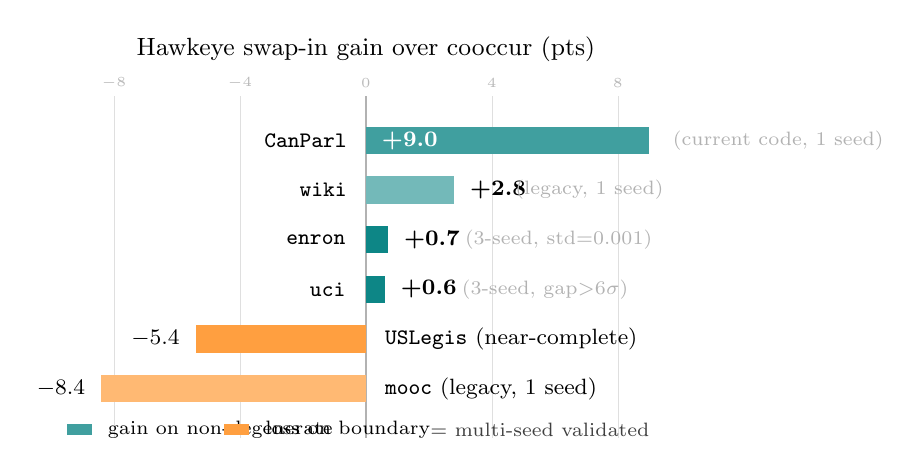
\begin{tikzpicture}[every node/.style={font=\footnotesize},x=0.4cm,y=0.7cm]
  % --- grid + axis ---
  \foreach \x in {-8,-4,0,4,8}{%
    \draw[gray!25,very thin] (\x,0.4) -- (\x,-5.8);%
    \node[gray!55] at (\x,0.65) {\tiny $\x$};}
  \draw[gray!60, line width=0.6pt] (0,0.4) -- (0,-5.8);
  \node[anchor=south] at (0,0.85) {\small Hawkeye swap-in gain over cooccur (pts)};

  % CanParl +9.0 (current code, single seed — multi-seed sweep running)
  \fill[teal!75]  (0,-0.15) rectangle (9.0,-0.65);
  \node[anchor=west,white] at (0.2,-0.4) {\textbf{+9.0}};
  \node[anchor=east] at (-0.3,-0.4) {\texttt{CanParl}};
  \node[anchor=west,gray!60] at (9.2,-0.4) {\scriptsize\ (current code, 1 seed)};

  % wiki +2.8 (legacy single-seed)
  \fill[teal!55]  (0,-1.05) rectangle (2.8,-1.55);
  \node[anchor=west] at (3.0,-1.3) {\textbf{+2.8}};
  \node[anchor=east] at (-0.3,-1.3) {\texttt{wiki}};
  \node[anchor=west,gray!60] at (4.2,-1.3) {\scriptsize\ (legacy, 1 seed)};

  % enron +0.7 (3-seed multi-seed verified)
  \fill[teal!95]  (0,-1.95) rectangle (0.7,-2.45);
  \node[anchor=west] at (0.9,-2.2) {\textbf{+0.7}};
  \node[anchor=east] at (-0.3,-2.2) {\texttt{enron}$^{\bigstar}$};
  \node[anchor=west,gray!60] at (2.6,-2.2) {\scriptsize\ (3-seed, std$=$0.001)};

  % uci +0.6 (3-seed multi-seed verified)
  \fill[teal!95]  (0,-2.85) rectangle (0.6,-3.35);
  \node[anchor=west] at (0.8,-3.1) {\textbf{+0.6}};
  \node[anchor=east] at (-0.3,-3.1) {\texttt{uci}$^{\bigstar}$};
  \node[anchor=west,gray!60] at (2.5,-3.1) {\scriptsize\ (3-seed, gap$>$6$\sigma$)};

  % USLegis -5.4 (boundary)
  \fill[orange!75]  (-5.4,-3.75) rectangle (0,-4.25);
  \node[anchor=east] at (-5.6,-4.0) {\textbf{$-5.4$}};
  \node[anchor=west] at (0.3,-4.0) {\texttt{USLegis} (near-complete)};

  % mooc -8.4 (legacy)
  \fill[orange!55]  (-8.4,-4.65) rectangle (0,-5.15);
  \node[anchor=east] at (-8.6,-4.9) {\textbf{$-8.4$}};
  \node[anchor=west] at (0.3,-4.9) {\texttt{mooc} (legacy, 1 seed)};

  % --- legend ---
  \fill[teal!75] (-9.5,-5.75) rectangle (-8.7,-5.55);
  \node[anchor=west] at (-8.5,-5.65) {\scriptsize gain on non-degenerate};
  \fill[orange!75] (-4.5,-5.75) rectangle (-3.7,-5.55);
  \node[anchor=west] at (-3.5,-5.65) {\scriptsize loss on boundary};
  \node[anchor=west,gray!50!black] at (1.5,-5.65) {\scriptsize $\bigstar$ = multi-seed validated};
\end{tikzpicture}
